% Part 1: Technical Landscape
\section{Technical Landscape}

\begin{frame}
\frametitle{Transformer Architecture}
\begin{itemize}
    \item \textbf{"Attention is All You Need"} (Vaswani et al., 2017)
    \item Self-attention mechanism: captures long-range dependencies
    \item Key components:
    \begin{itemize}
        \item Multi-head attention
        \item Positional encoding
        \item Feed-forward networks
        \item Layer normalization
    \end{itemize}
    \item Advantages:
    \begin{itemize}
        \item Parallel processing (vs. sequential RNNs)
        \item Flexible context modeling
        \item Scalable architecture
    \end{itemize}
\end{itemize}
\end{frame}

\begin{frame}
\frametitle{Probabilistic Modeling}
\begin{itemize}
    \item Language modeling as probability distribution: $P(w_1, w_2, ..., w_n)$
    \item Autoregressive formulation: $P(w_t | w_1, ..., w_{t-1})$
    \item Training objectives:
    \begin{itemize}
        \item Autoregressive language modeling
        \item Masked language modeling
        \item Diffusion models
    \end{itemize}
    \item Maximum likelihood estimation via cross-entropy loss
    \item Foundation for generation and understanding
\end{itemize}
\end{frame}

\begin{frame}
\frametitle{Scaling Laws}
\begin{itemize}
    \item \textbf{Key insight}: Model performance scales predictably with:
    \begin{itemize}
        \item Model size (parameters)
        \item Dataset size (tokens)
        \item Compute budget (FLOPs)
    \end{itemize}
    \item Power law relationships (Kaplan et al., 2020)
    \item Chinchilla scaling laws (Hoffmann et al., 2022):
    \begin{itemize}
        \item Optimal ratio of model size to training data
        \item Compute-optimal training
    \end{itemize}
    \item Implications: Bigger models, more data = better performance
\end{itemize}
\end{frame}

\begin{frame}
\frametitle{Emergent Abilities}
\begin{itemize}
    \item Capabilities that appear at scale, absent in smaller models
    \item Examples:
    \begin{itemize}
        \item Few-shot learning (GPT-3)
        \item Chain-of-thought reasoning
        \item Instruction following
        \item Multi-step problem solving
        \item Arithmetic and symbolic reasoning
    \end{itemize}
    \item Not explicitly trained, emerge from scale
    \item Phase transitions in capability vs. scale
    \item Critical for advanced applications
\end{itemize}
\end{frame}

\begin{frame}
\frametitle{LLM and Agent Development Roadmap}
\begin{center}
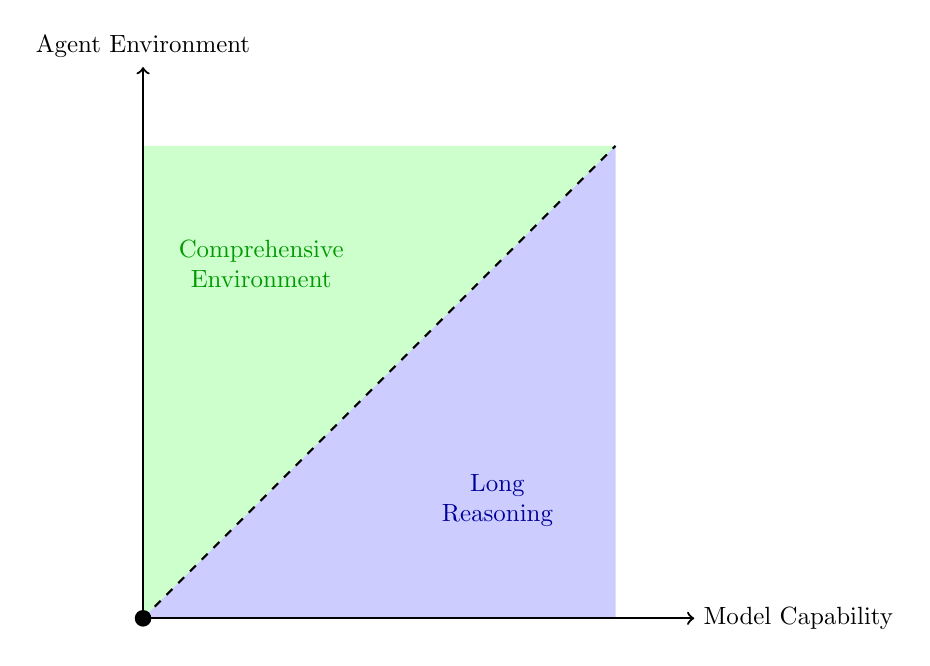
\begin{tikzpicture}[scale=1.0, every node/.style={scale=0.9}]
    % Define the size of the square
    \def\maxsize{6}
    
    % Fill upper-left triangle (Comprehensive Environment)
    \fill[green!20] (0,0) -- (0,\maxsize) -- (\maxsize,\maxsize) -- cycle;
    
    % Fill lower-right triangle (Long Reasoning)
    \fill[blue!20] (0,0) -- (\maxsize,0) -- (\maxsize,\maxsize) -- cycle;
    
    % Draw the diagonal line y=x
    \draw[thick, dashed] (0,0) -- (\maxsize,\maxsize);
    
    % Axes
    \draw[->, thick] (0,0) -- (\maxsize+1,0) node[right] {Model Capability};
    \draw[->, thick] (0,0) -- (0,\maxsize+1) node[above] {Agent Environment};
    
    % Origin point (without text label)
    \fill (0,0) circle (3pt);
    
    % Labels for regions
    \node[green!60!black, align=center] at (1.5,4.5) {Comprehensive\\Environment};
    \node[blue!60!black, align=center] at (4.5,1.5) {Long\\Reasoning};
\end{tikzpicture}
\end{center}
\end{frame}
